%%%%%%%%%%%%%%%%%%%%%%%%%%%%%%%%%%%%%%%%%%%%%%%%%%%%%%%%%%%%%%%%%%%%%%%%%%%%%
\section{Examples of OpencCL Applications}


%------------------------------------------------------------------------------
\subsection{OpenCL on FPGA platforms}

\subsubsection{OpenCL-FPGA Implementation}
As we already saw, OpenCL applications consists of two part: the host and the kernels.
FPGA flexibility allow the developer to opt for two solutions:

\begin{enumerate}
	\item An "`All in One"' solution, by implementing the CPU that will run the standard C/C++ host code directly as a soft CPU inside the FPGA.
	\item A separate solution, by using an external microprocessor for the host and by programming the FPGA to execute the kernels only.
	\end{enumerate}
	
Unlike CPUs and GPUs, where parallel threads can be executed on different cores, FPGAs offer a different strategy. Kernel functions can be transformed into dedicated and deeply pipelined \textbf{hardware circuits} that are inherently multithreaded using the concept of pipeline parallelism. Each of these pipelines can be replicated many times to provide even more parallelism than is possible with a single pipeline. This translates in an immediate boost in performance.\\
Figure \ref {fig:fpga_example} shows a simple example of how kernels are translated into separate \textbf{hardware pipelines}.
	
\begin{figurehere}
 \centering
 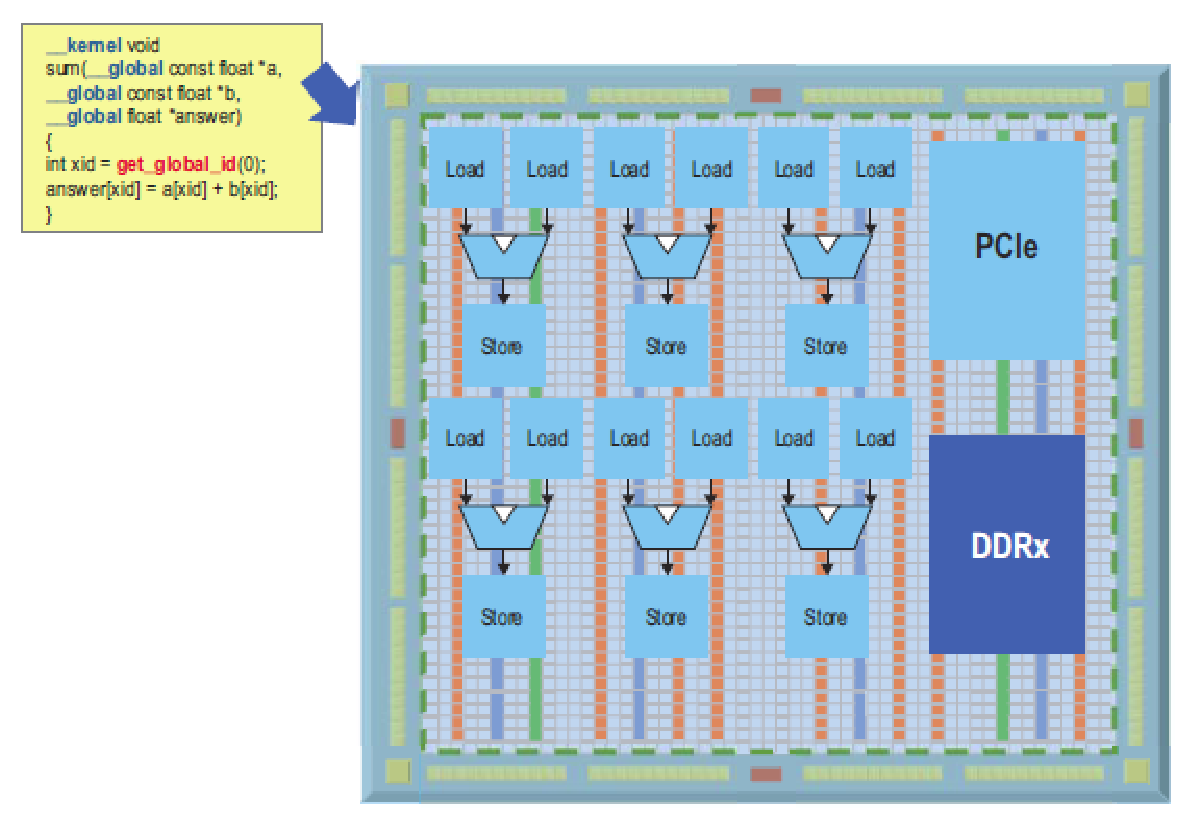
\includegraphics[width=8cm, height=4cm]{./eps/FPGA1.eps}
 \caption{FPGA implementation example}
 \label{fig:fpga_example}
\end{figurehere}

The most important concept behind the OpenCL-to-FPGA compiler is the notion of \textbf{pipeline parallelism}.
Basically, an OpenCL-to-FPGA compiler is able to implement the scenario observed in Section \ref{sect:pipelineScenario} in an automatic and more efficient way. We will describe how pipeline parallelism work by introducing an example, shown in Figure \ref{fig:fpga_example2}:

\begin{figurehere}
 \centering
 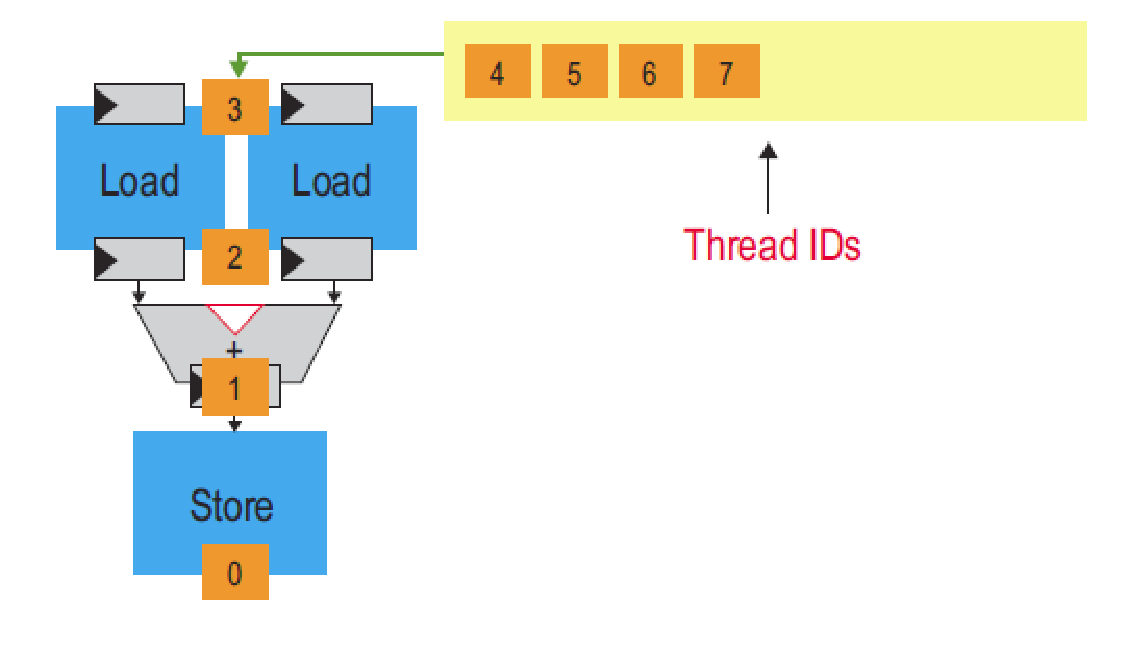
\includegraphics[width=8cm, height=4cm]{./eps/FPGA2.eps}
 \caption{Pipeline parallelism example}
 \label{fig:fpga_example2}
\end{figurehere}

On the first clock cycle, thread 0 is clocked into the two load units. This indicates that they should begin fetching the first elements of data from arrays A and B. On the second clock cycle, thread 1 is clocked in
at the same time that thread 0 has completed its read from memory and stored the results in the registers following the load units. On cycle 3, thread 2 is clocked in, thread 1 captures its returned data, and thread 0 stores the sum of the two values that it loaded. It is evident that in the steady state, all parts of the pipeline are active, with each stage processing a different thread.
	
To complete this section, we'll present a general scheme that summarize how OpenCL-FPGA applications are implemented (Figure \ref{fig:fpga_implementation}). One crucial point for parallel computation is the memory management, and as we can see from the figure several memory interfaces are needed, but luckily OpenCL-FPGA compilers are usually able to implement such interfaces automatically.

\begin{figurehere}
 \centering
 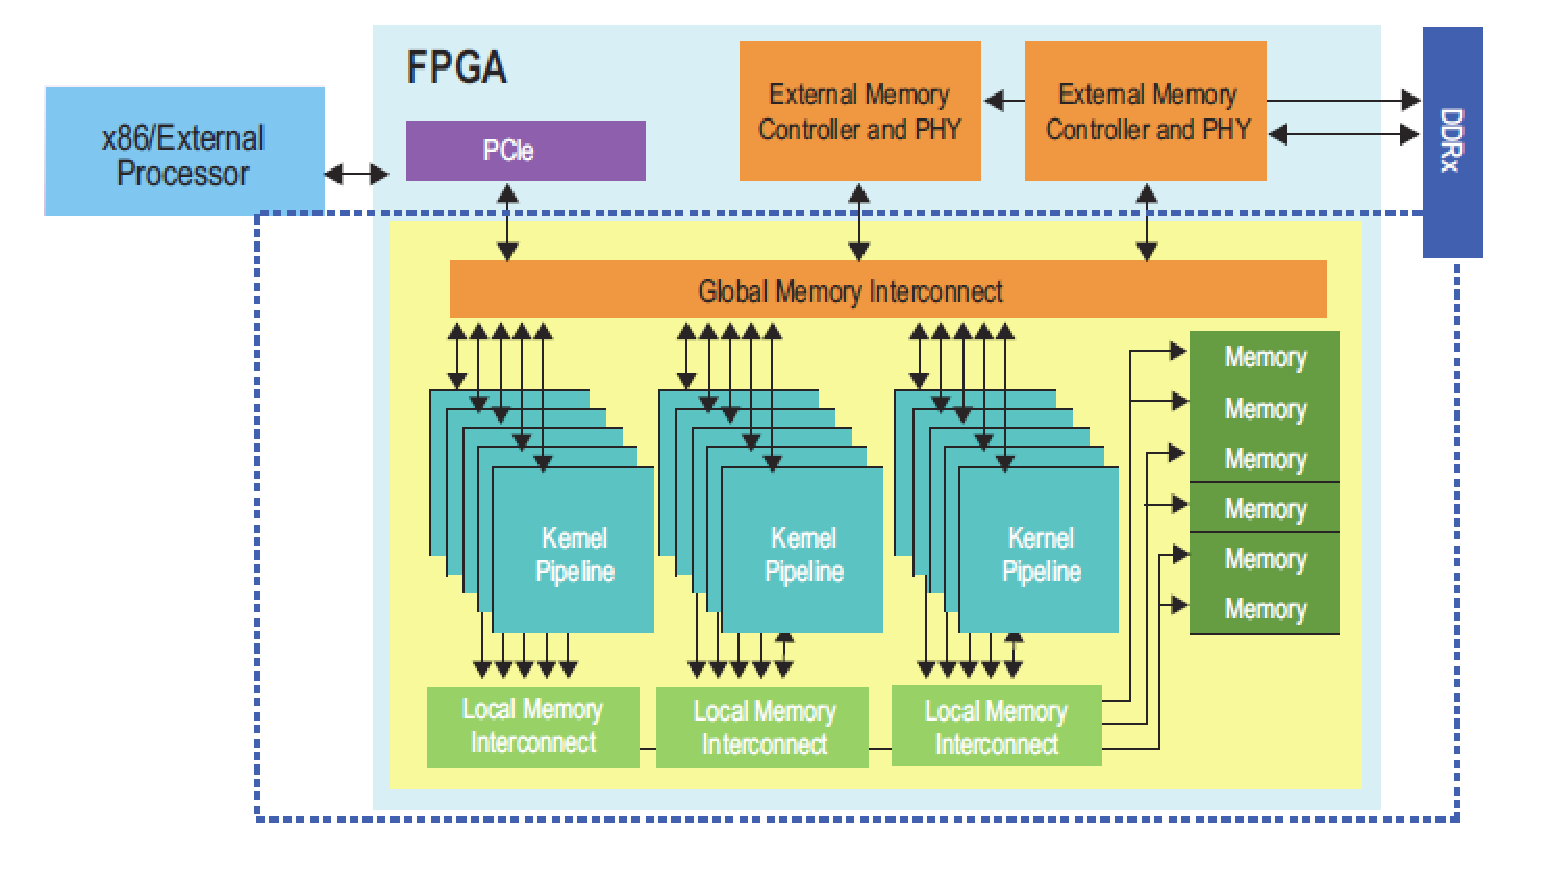
\includegraphics[width=8cm, height=4cm]{./eps/FPGA3.eps}
 \caption{OpenCL-FPGA Implementation scheme}
 \label{fig:fpga_implementation}
\end{figurehere}

\subsubsection{Benefits}

\begin{itemize}
	\item \textbf{Improved Time To Market:} OpenCL offers a quicker and simpler way to implement parallel alghorithms  compared to traditional FPGA development using lower level hardware description language (HDLs) such as Verilog or VHDL \cite {altera:FPGA}.  This because OpenCL inherently offers the ability to describe parallel computation, while the main challenge in HDLs languages was exactly to extract thread-level parallelism from a sequential program. OpenCL offers instead the ability to the programmer to explicitly specify and control parallelism.
\end{itemize}


%-----------------------------------------------------------------------------



